\documentclass[../thesis]{subfiles}
\begin{document}

\chapter{Background}

A growing body of work in the field of meta-research has identified a
number of obstructions to research reproducibility and possible
techniques for improving the trustworthiness of scientific
publications. One promising approach for addressing some of these
factors is the widespread adoption of standardized procedures for
experiment design, record keeping, and publication, supported wherever
possible by software tools for automation and research life cycle
management. This chapter identifies the functional requirements of a
software system for designing and executing complex experiments and
organizing their results and justifies the need for a next-generation
collaborative lab information management system. We briefly describe
the electrochemical sensor research which produced our group's need
for the software, analyze the tooling requirements of our project, and
then explore the existing ecosystem of software tools for automation
and curation of research.



\section{Use case: Electrochemical sensor arrays}

Our development of a next-generation collaborative \gls{LIMS} is
motivated by a concrete research task, namely characterization and
design of electrochemical sensor arrays for precise concentration
estimation of a broad range of chemical targets \cite{Li2014,
  Wang2016, Wang2014}. Electrochemical sensors are sensitive to a
number of interacting environmental conditions such as temperature,
humidity, ambient airflow, and presence of trace interferent chemicals
\cite{Marco2012}. The sensitivity of a given sensor to a particular
analyte compound is also a complex function of device geometry,
electrolyte and substrate materials, and applied electrical
stimulus. In order to make measurements meaningful, as much of this
secondary information as possible must be collated with the raw
electrical output of the sensors. Additionally, a typical
characterization experiment involves a sequence of manipulations of
controllable parameters such as the flow rates of input gases or
applied voltage waveforms. The end engineering goal of these
experiments is to determine the inverse function mapping each sensor's
instantaneous output current, input voltage, and observable
environmental parameters into a concentration profile of the device's
chemical environment. For an experimental data set to afford such an
analysis, the input conditions should be controlled as accurately as
possible, and especially for batteries of tests involving many sensors
operating in tandem it is necessary to employ computer control to
achieve uniform results.

This experimental scenario, depicted schematically in figure
\ref{fig:EchemSetup},
will serve as a running example to demonstrate the
capabilities and requirements of the software tool described by this
thesis. Our ideal experimental setup involves commercial lab equipment
as well as custom data acquisition hardware, simultaneous operation of
many sensors with different physical characteristics, and precisely
timed computer choreography of electrical interrogation protocols and
gas flow rates. Furthermore, the exact nature of the experiments being
run changes frequently as researchers identify new questions, design
new sensors, and involve new equipment in their work,
requiring our control and data management software to grow with the
changing requirements of its users.

We believe that a software framework capable of scheduling and
autonomously executing experiments of this level of complexity has the
potential to be more broadly useful in any scientific environment with
similar workflow needs. By generalizing our design from this use case,
we hope to meet our project's needs and simultaneously provide the
research community with powerful, much-needed open-source solutions
for a set of problems that recur in many different scientific areas.
The design goals of our software package are enumerated in the
following section, followed by an overview of the existing tools which
fulfill some of these requirements.

\begin{figure}
  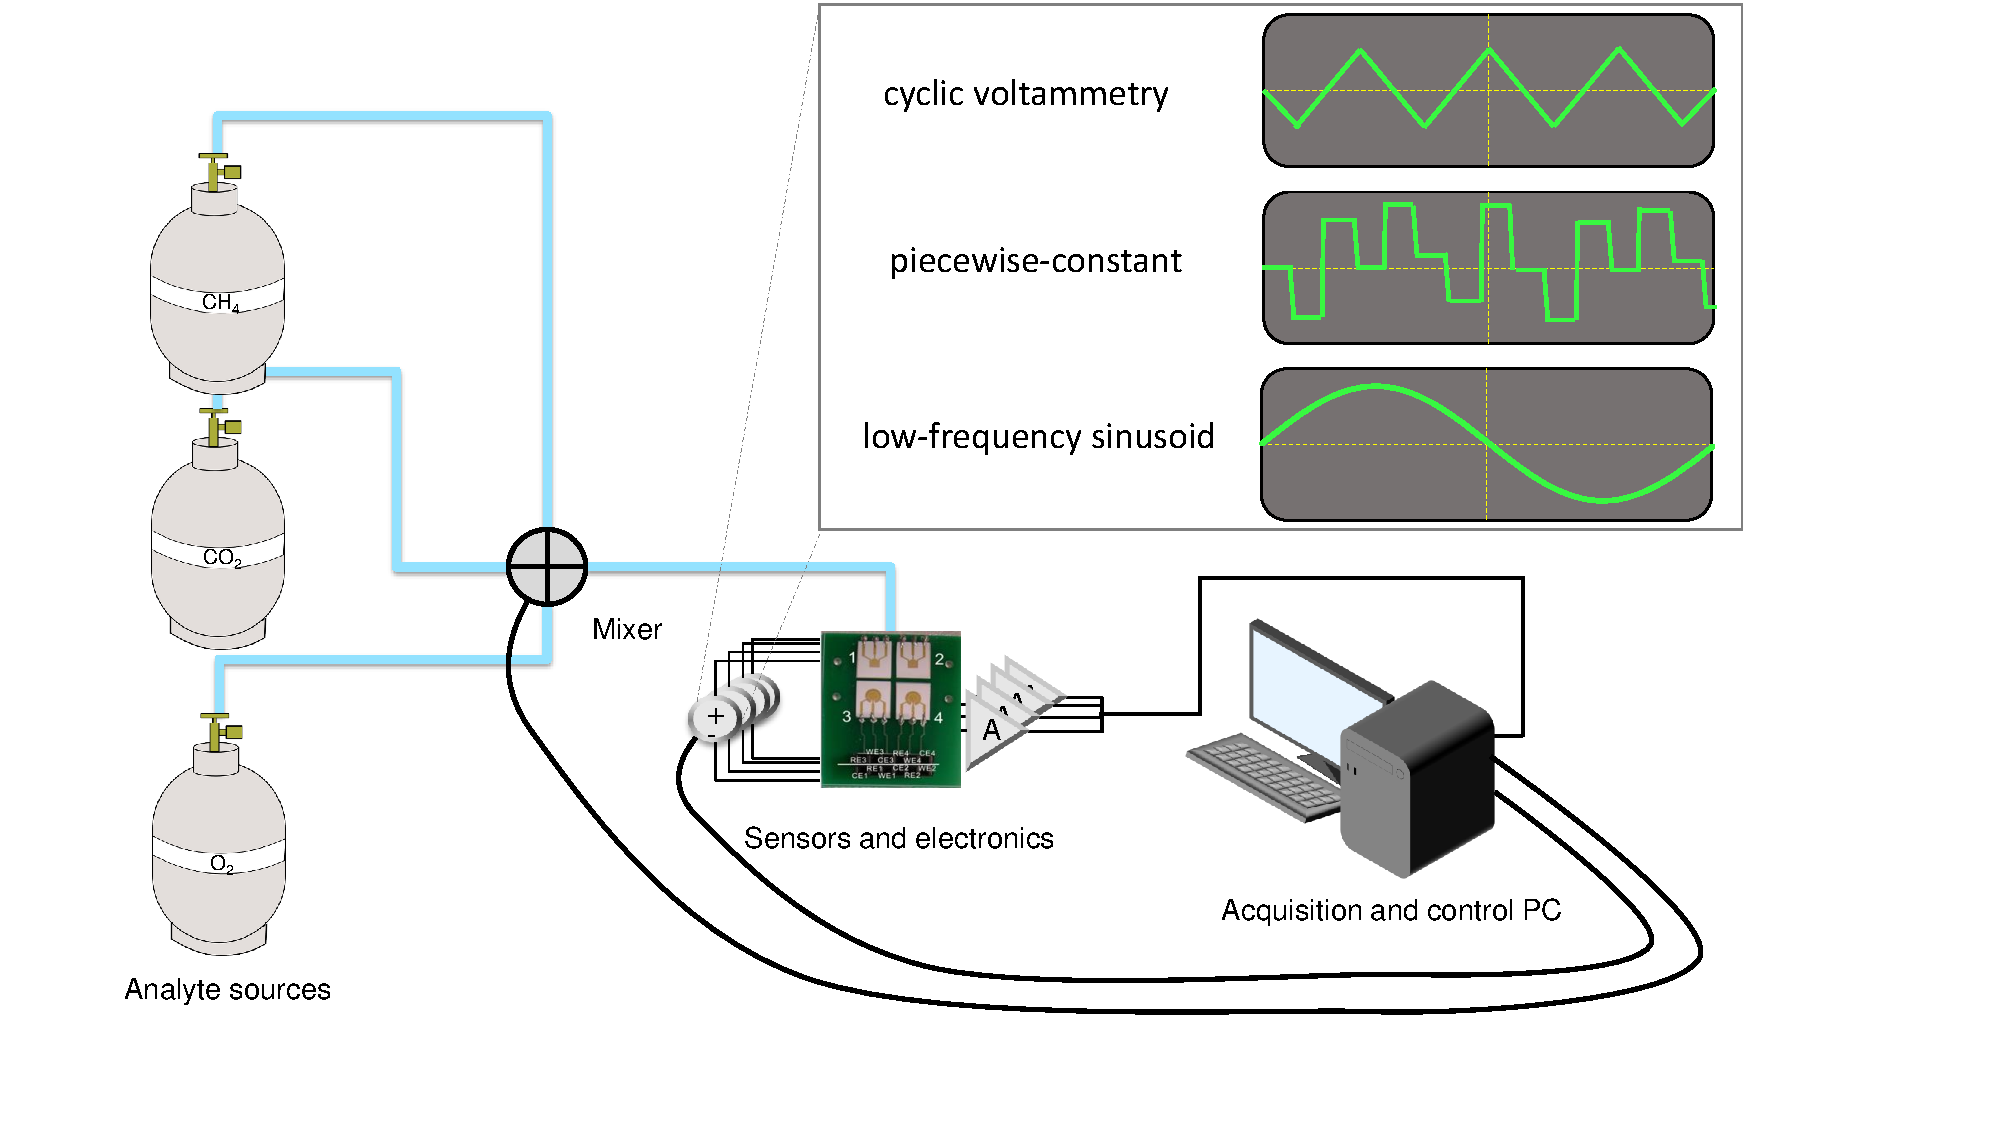
\includegraphics[width=\textwidth]{echem-setup}
  \caption{
    Schematic of an example experimental apparatus for
    characterizing an array of electrochemical gas sensors.
    Inset: some commonly used stimulus waveforms for interrogating
    electrochemical sensors.
    \label{fig:EchemSetup}
  }
\end{figure}



\section{Requirements and Terminology}
Laboratory science presents a diverse set of operations management and
informatics challenges, and many research reproducibility efforts stand to
benefit from carefully designed software tools. In this section we
consider some of the many scalability challenges faced by a typical
research group and examine some proposed techniques for addressing
them. This discussion has guided the design of the software framework
presented later in this thesis.

\subsection{Automation}
The desire to scale experiments to much higher throughput provides a
major motivation for exploring software solutions for lab management.
As researchers begin to work with many devices and control
parameters simultaneously, data collection and tracking tasks become
difficult to manage. Additionally, when attempting to provide
confident analyses of large sensor characterization data sets, signal
processing experts require accurate information about the timing of
input and output events, and adequate resolution of control events is
extremely difficult to obtain under manual operation.

By employing computer control of actuators and data collection
equipment whenever possible, researchers should be able to maximize
the consistency of their results while simultaneously
improving their productivity. The ability to automatically re-run a
task with modified parameters overnight rather than carefully
manipulating control dials for hours on end would allow scientists
to focus their expertise on identifying new research questions rather
than on tedious and meticulous experiment execution.
An ideal software tool for lab automation should allow investigators
to design, refine, and compose executable tasks, enabling researchers
to build complex experimental protocols from a library of reusable
components.

\subsection{Metadata and data provenance}
Much of the data that is collected and exchanged by researchers is
stored in ad-hoc file formats, often detached from the relevant
metadata necessary to make these results meaningful. Examples of
metadata which are often omitted from raw data sets include
measurement units, input conditions, sample and equipment IDs, and
annotations such as the hypothesis of an experiment or where to find
further documentation or references. These key pieces of information
are often recorded or remembered only by the original experimenter and
may easily become unavailable to future researchers.
Even when data collection and management policies are established within
a group, it requires careful discipline to enforce these
rules manually, especially in a typical fast-paced research
environment with little direct oversight.

Furthermore, in many cases drawing conclusions about a data set relies on
information about experimental conditions that is
difficult to acquire for every trial and is not obviously
relevant at the outset, forcing researchers to backtrack and repeat
work in order to be confident in their results. By using software to
collect and manage information about the flow of data through an
experiment, users can be provided with powerful tools for examining
their workflows at many levels of detail without requiring costly and
time-consuming repeat trials.

Systematically tracking and organizing the history of data sets as
they are collected, reformatted, and undergo transformations and
analysis is the focus of the growing area of \gls{dataProvenance} \cite{buneman2000data}.
Provenance techniques aim to allow researchers to properly attribute a
data set, understand how it was created, and determine where and how
modifications or errors were introduced. Capturing and serializing
accurate and sufficient provenance information about a system remains
a research topic of its own \cite{Cheney:2009:PFH:1639950.1640064},
but a number of existing scientific software tools provide some
features that cater to this need.

\subsection{Version control}
Whenever software provides the ability to create and modify complex
documents or \glspl{artifact}, version control
is a valuable feature for improving productivity and
auditability. Similar in concept to \gls{dataProvenance}, a \gls{VCS}
keeps checkpoints of important points in a file's edit history,
allowing authors to review past states, recover lost work, and make
changes to a single file rather than attempting to manually keep track
of backups. Version control tools are indispensable in the software
industry for tracking source code, where popular tools include Git
\cite{Git} and Subversion \cite{Subversion}, but some version control features are
now commonplace in office programs such as Microsoft Word's ``Track
Changes'' mode \cite{Word}. Existing version control software for plain
text files is extremely mature, full-featured, and powerful, and may
be used as a third-party tool for any work where plain text code and
configuration files are \glspl{artifact} of interest.

\subsection{Collaboration}
Modern research labs are increasingly interdisciplinary and rely on
remote sharing of techniques, data, and publications. Software
designed for assisting researchers with performing and documenting
their work should reflect these realities, ideally offering native
support for sharing and collaboratively reviewing resources over the
Internet. Software systems with distribution in mind are also well
equipped to enforce policies about data usage and to maintain
end-to-end provenance information about \glspl{artifact} by managing records
in a server-side database. Furthermore, the use of electronic media
enables users to assemble information-rich dissemination units, and
software which supports portable and information-dense file formats
provides benefits for long-term collaboration as well as publication.

\subsection{Extensibility}
A common user complaint about commercial software with proprietary
code bases is that tools are overly rigid and ill-suited for adapting
to the rapidly changing needs of users \cite{morgan2007benefits}.  The
fast pace and necessary interaction with bleeding-edge technologies
provides one possible reason for the proliferation of lab management
software packages with slightly different goals and feature sets. To
address this problem, we feel that researchers should be allowed and
encouraged to customize and modify their lab management software to
meet their needs. Open-source projects are theoretically arbitrarily
extensible, since users may directly modify the software, but in many
cases open source tools are still not designed with customization in
mind. Systems with a modular design that support community-crafted
plugins, user-level scripting, and straightforward integration with
third-party tools are able to grow alongside users' changing needs and
allow dedicated users to compound the initial learning investment over
time. Such systems, when well-designed, often benefit from greater
longevity and feature-richness than traditional monolithic programs
\cite{Emacs, SuperCollider}.

\subsection{User compliance}
A known challenge faced when developing software for applications such
as reproducible research is that feature-rich tools often present users
with a substantial learning curve, deterring widespread
adoption. Tools which do not confer an obvious
advantage immediately or disrupt users' existing workflows are likely
to go unused, wasting development effort. Research on the topic
suggests that ease of use and accessibility of documentation are
important concerns for promoting user adoption
\cite{Lederer2000}. Usability can also be improved and demonstrated by
providing concrete examples of how the software can solve problems
faced routinely by domain scientists and encouraging users to tailor
the tools to their unique preferences and needs. Other important
determinants of user compliance include upgradability, technical
support, reliability, and compatibility with existing tools
\cite{wang2001open}. Addressing user experience concerns from the
outset of a design and incorporating feedback in the development
process can result in an ultimately richer product, and this is one of
the key insights of the now-popular Agile development methodology
\cite{begel2007usage}.

\subsection{Security}
Intellectual property is an important issue in both industrial and
academic research, given that funding, commercial competitiveness, and
legal and professional recognition are often contingent on
\gls{scientificPriority}. Internet-connected software which manages
potentially sensitive data and design documents must therefore make
digital security a principal concern. An architecture for online
experiment analysis and design must carefully conform to the latest
security best practices and maintain careful access controls while
allowing for collaboration.

\section{Review of existing experiment management \mbox{software}}

The complex needs of modern research have created a large specialized
software market, and there are now dozens of tools for computerizing
various laboratory management and research tasks. There are now many
companies offering lab informatics software with a broad range of
capabilities. Since many of these programs are proprietary, it is
difficult to compare their feature sets precisely, and many
packages are defunct or poorly documented. Below we attempt to provide a
broad overview of the major classes of software most aligned with our
goals, giving a few examples of prominent products in each category.

\subsection{Electronic lab notebooks}
An \gls{ELN} is a software tool for helping
researchers to chronicle their day-to-day investigations and
results. A typical \gls{ELN} package allows researchers to compose
rich-text documents consisting of text and figures alongside technical
\glspl{artifact} such as data tables. Several surveys of
commercially available ELNs have been published
\cite{Rubacha2011, Dirnagl2016}, but the domain is still evolving
rapidly and some of these programs have begun to integrate complex
capabilities such as version control, experiment specification, and
more. Many of the commercial products in this domain
offer users compliance with the FDA's recommendation on electronic
record keeping \cite{FDA}, a set of guidelines promoting thorough,
auditable documentation of research performed in the agricultural and
health sectors.

\begin{figure}
  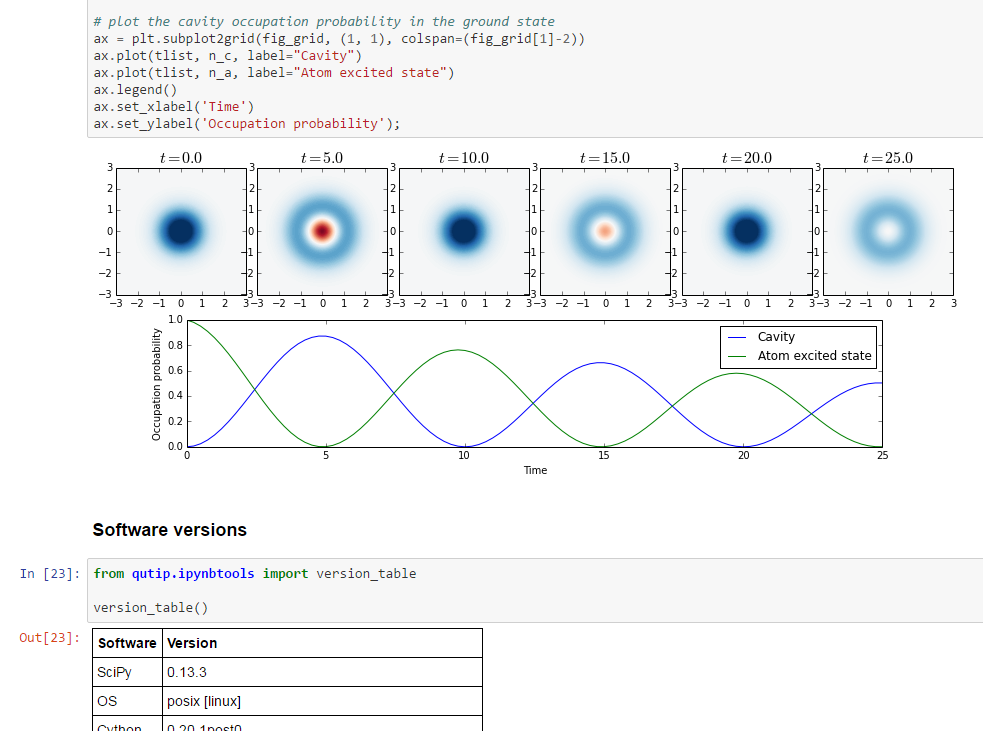
\includegraphics[width=\textwidth]{ipython}
  \caption{
    An electronic lab notebook page in IPython/Jupyter v4.1.0
    \cite{IPython} integrating documentation, code, inline math,
    and figures.
    \label{fig:Ipython}
  }
\end{figure}

Most general-purpose programming language environments targeted toward
scientific computing now include some degree of ELN
functionality. These tools are typically environments for literate
programming \cite{Knuth:1984:LP:473.479} which are able to embed plots
and data tables alongside code and natural language
documentation. Popular solutions in this domain include Mathematica
\cite{mathematica}, R \cite{Rlang}, IPython/Jupyter \cite{IPython},
and MATLAB Notebook \cite{MATLAB}.

\subsection{Workflow design tools}
Defining, composing, and documenting complex procedures is a core
organizational need of many research groups. A number of so-called
\glspl{workflowMgmt} have emerged to help manage task schedules and
dependencies in domains such as manufacturing
\cite{Allweyer:2010:BPM:1841147}, high performance computing
\cite{VisTrails}, and business management
\cite{cardoso2004workflow}. Workflow editors provide users with a
means of constructing executable tasks by describing how
data moves through them, typically by visually manipulating a directed
graph of processes as in figure \ref{fig:TavernaWorkflow}. In some
cases workflows may serve purely as
documentation, while workflow tools for \textit{\gls{insilico}} science
are often executable and may be bundled with data to provide direct
replication of analysis flows on other machines. The most prominent
examples of workflow software
targeted toward scientists are built to facilitate the design and
execution of high performance computing simulations such as Apache
Taverna \cite{Taverna} and VisTrails \cite{VisTrails}. Less
attention has paid to scientific processes that are not completely digital
and are therefore harder to fully automate. The application
of similar software to managing business processes and software
development suggests that these tools may also be valuable aids for
describing complicated scientific experiments, and some \gls{LIMS} packages
provide some of this functionality \cite{CoreLIMS}. By combining these
workflow specification tools with software for controlling lab
equipment, it may be possible to provide domain scientists with a
powerful framework for defining executable specifications of
complicated laboratory procedures.

\begin{figure}
  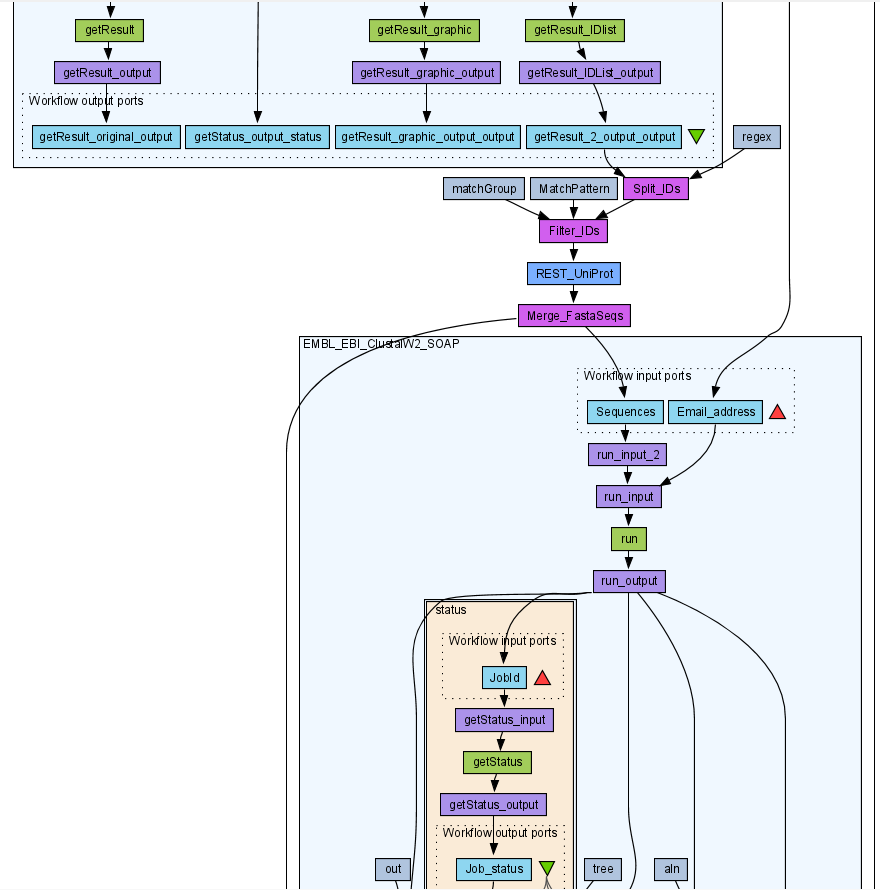
\includegraphics[width=\textwidth]{taverna-workflow}
  \caption{
    Editing a protein sequence analysis workflow
    (retrieved from \cite{ExampleWorkflow}) in
    Apache Taverna v2.5 \cite{Taverna}, an open-source workflow
    management tool.
    \label{fig:TavernaWorkflow}
  }
\end{figure}

A related class of software reproducibility tools encourages users to
bundle input sets and sequences of data-transforming programs into a
single distributable file intended to accompany published results.
A notable example is \cite{ReproZip}, which uses virtual machines to
produce self-contained computing environments for reproducing digital
analysis under identical conditions on different physical
computers. ReproZip automatically determines all the files necessary
for replicating an \textit{\gls{insilico}} workflow by monitoring the operating
system during ordinary task execution. These techniques offer a
promising strategy for improving scientists' ability to capture the
intricacies of their work for later review or reuse while avoiding
excessive demands on the user's discipline.

Industry groups have also made several attempts to produce
standardized data models for business processes and equipment, perhaps
the most popular of which is \gls{BPMN}
\cite{Allweyer:2010:BPM:1841147}, typically represented by a directed
graph or flowchart much like the data models used in scientific
workflow software. The
most full-featured model expanding on this concept is ISO 15926
\cite{West2009}. This model promises
a level of generality that is sufficient to enable interoperability
between businesses in different sectors and countries which rely on
large, varied sets of equipment and software. The still-growing
specification encompasses information as diverse as process
specification and refinement, structural description of organizations
and devices, component life cycle information and more. ISO 15926's
representation format is based on semantic web technologies such as OWL, which
employs a graph model to describe semantic relationships between
entities, where each entity and relationship has an associated
hyperlink. The standard has been under development for 25 years, but
many specification documents have yet to be published and no software
implementations are currently freely available. The extreme complexity
of the model is also an impediment to adoption by end users as well as
implementation.

\subsection{\Gls{LIMS}}
A \gls{LIMS} is a tool for tracking the operations and assets
of a laboratory. Commercial tools by this name provide a wide range
of features targeted toward different aspects of an enterprise-level
industrial lab such as letting researchers monitor their ongoing
experiments, logging samples and data sets, and notifying relevant
personnel when maintenance tasks like restocking need their
attention. This field is now occupied by a staggering number of
application vendors and products with a broad range of
specializations, feature sets, maturity levels, and price tags
\cite{LIMSWikiList}. These packages range from glorified
wiki/spreadsheet tools to specialized systems for interacting with
specific types of chemical analysis equipment.
Some \gls{LIMS} packages provide a \gls{workflowMgmt}
and many of them contain built-in \gls{ELN}s.

The primary players in this application domain target the needs of
labs in the healthcare, forensics, and pharmaceutical sectors and are
mostly designed for managing and optimizing huge batch processes on
fixed, well-defined equipment pipelines. The designs resulting from
these assumptions would seem to make many of these programs a poor fit
for the rapidly evolving experimental workflow seen in academic sensor
engineering, though there are exceptions.
In particular, Agilent's OpenLAB suite (formerly Kalabie)
\cite{OpenLAB} offers a notebook tool which combines data collection,
storage, analysis, and collaboration capabilities. This package is
also capable of integrating with data collected from instruments
manufactured by Agilent and some of its business partners. The tool
appears to provide many of the capabilities found in a typical
\gls{LIMS} combined with some support for real-time hardware control,
making it an attractive candidate for meeting several of our
application's needs. Unfortunately, this tool is restricted to a
specific set of associated hardware and at the time of this writing
lacks desirable features such as modularity, user-customizability, and
version control.

Most \gls{LIMS} toolkits are proprietary and closed-source, but given the
demand for this type of application from large industrial groups the
field is in some ways fairly mature. Some of the architectural
decisions that are commonplace in modern \gls{LIMS}, especially their
cloud-oriented model, support for user customization, and focus on
auditability, seem well-suited
for the kind of end-to-end research management system we intend to
build. Throughout this thesis we refer to the software tool we are interested
in building as a \gls{LIMS} due to the broad range of
functionality seen in tools which label themselves in this way.

\subsection{Equipment automation tools}
To extend automation of scientific processes beyond the purely
computational domain, several vendors offer tools for coordinating
simultaneous operation of actuators and data acquisition modules.
Likely the most visible software package providing this functionality
is National Instruments LabVIEW \cite{ELLIOTT2007}
LabVIEW's G visual programming language allows users to connect
devices, signal processing blocks, and graphical interface elements,
ultimately building a custom front panel and controller for a
``virtual instrument'' (VI) which may communicate with many different
pieces of lab equipment. LabVIEW interacts with National Instruments'
line of data acquisition and control hardware and also ships with a
large library of drivers for scientific instruments produced by many
vendors. G programs can be regarded to some degree as workflow-style
executable process specifications, but different versions of LabVIEW
have well-documented compatibility problems, preventing VIs from
serving as self-contained process dissemination units.

Other software toolkits have begun to capitalize on
the recent emergence of affordable network-connected microcontrollers
and single-board computers. One toolkit overlapping with some
of our application requirements, ZettaJS, intends to provide a
hardware abstraction layer for controlling and coordinating embedded
data acquisition platforms over the web \cite{ZettaJS}, with the
stated goal of connecting devices to the \gls{IoTg} using existing web
technologies.

Unfortunately, relatively few \gls{LIMS} vendors incorporate equipment
automation into their feature sets. Even fewer packages seem to
recognize the ways \gls{ELN} capabilities could be complemented by
end-to-end experiment design and execution support. We feel that there
is a promising niche for software synthesizing the best features of
automation software, cloud-based \gls{LIMS}, and metadata-rich
\gls{ELN}, and this thesis intends to articulate the design of such a
framework.



\section{Rich publication data models}
A core component of a software system for experiment management is its
model for representing research \glspl{artifact}. Knowledge
engineering and data archiving researchers have proposed several
approaches for representing the broad space of research-relevant
information in a machine-readable form, and some of these models are
recognized in this section.

\subsection{Semantic provenance models}
Academic work on structured representations of research artifacts,
their relationships, and their provenance has largely built on
semantic web technologies such as the so-called linked data network
\cite{LinkedData}. Linked data calls for scientific resources on the
web to include hyperlinks to semantically related external pages. In
particular, this provides a mechanism for published data sets to
record their provenance by explicitly stating a chain of relationships
to their point of creation. A standards-track recommendation endorsed
by the the World Wide Web Consortium known as W3C PROV \cite{PROV} has
recently been developed to specify how dissemination units should
identify their influences. Semantic web technology has enjoyed many
years of academic development and resulted in some promising
high-profile projects such as DBpedia \cite{DBpedia}. However,
criticism of the semantic web's vision and approach has been readily
available throughout its long history
\cite{Marshall:2003:SW:900051.900063}, and due to a lack of interest
in the industry and open source software communities the tooling
support for developing cutting-edge web apps that rely on \gls{RDF}
metadata remains limited.

\subsection{Research objects}
A \gls{researchObject} is a proposed format for archiving scientific
data as well as an example of a richly annotated electronic
publication format \cite{bechhofer2010research}. Many of the existing
publications on the research object model use linked data technology
to encode relationships between the constituent artifacts of a
research object as well as between



\section{Summary}
A number of software tools for automating data collection, analyzing
and comparing data sets, and interdisciplinary scientific
collaboration have emerged in recent years. Many of these packages
provide much-needed informatics capabilities that are currently being
leveraged by both academic and industry labs, especially in the
biomedical and healthcare sectors. However, addressing the full set of
challenges posed by interdisciplinary high-throughput sensor research
and development will require the integration of \gls{LIMS}
functionality, an electronic notebook editor, and a scripting or
graphical programming solution for equipment automation into a
cloud-based software framework that currently does not exist. The
remainder of this thesis will describe the proposed design and
prototype implementation of a suite of software tools which
synthesizes and expands upon the programs described above.

\end{document}

%%% Local Variables: ***
%%% mode:latex ***
%%% TeX-master: "../thesis.tex"  ***
%%% End: ***